% Sample LaTeX file for creating a paper in the Morgan Kaufmannn two
% column, 8 1/2 by 11 inch proceedings format.

\documentclass[letterpaper]{article}
\usepackage{uai2019}
\usepackage[margin=1in]{geometry}

% Set the typeface to Times Roman
\usepackage{times}
\usepackage[utf8]{inputenc}
\usepackage{mathtools}
\usepackage{amsfonts}
\usepackage[colorlinks=true,citecolor=blue,urlcolor=blue]{hyperref}

\newcommand{\mean}[1]{\left\langle #1 \right\rangle}
\newcommand{\avg}[1]{\langle#1\rangle}
\newcommand{\et}{\;\mathrm{and}\;}
\newcommand{\Real}{\mathbb{R}}
\newcommand{\STAB}{\mathrm{STAB}}
\renewcommand{\TH}{\mathrm{TH}}

\title{Exclusivity graph approach to Instrumental inequalities}

%\author{Davide Poderini}
%\author{Iris Agresti}
%\author{Gonzalo Carvacho}
%\author{Fabio Sciarrino}
%\affiliation{Dipartimento di Fisica, Sapienza Universit\`{a} di Roma,
%Piazzale Aldo Moro 5, I-00185 Roma, Italy}
%
%\author{Rafael Chaves}
%\author{...}
%\affiliation{International Institute of Physics, Federal University of Rio %Grande do Norte, 59070-405 Natal, Brazil}
%\affiliation{School of Science and Technology, Federal University of Rio %Grande do Norte, 59078-970 Natal, Brazil}

\author{} % LEAVE BLANK FOR ORIGINAL SUBMISSION.
          % UAI  reviewing is double-blind.

\begin{document}

\maketitle

\begin{abstract}
\textcolor{blue}{Instrumental tests have been widely used to derive causal
   relations between variables even in presence of unobserved latent factors,
   thus providing a powerful tool for different sciences ranging from xxx to
   xxx. Recently, much interest have been dedicated to the instrumental scenario
   since admits quantum violations with fewer resources respect to the Bell
   analogue, this property can be exploited to (drastically?) improve our
   current capacities to process information. Dire qualcosa della contextuality.
   Here, we present the instrumental inequality under a contextual approach,
   showing that the geometry of correlations within this framework allow us to
   find optimal xxxxxxxxxxxxxxxxxxxxxxxxxxxxxxx  }  
\end{abstract}

\section*{Introduction}
Inferring  whether a variable $A$ is the cause of another variable $B$ is at the
core of causal inference. However, unless interventions are available
\cite{pearlbook}, one can cannot exclude that observed correlations between $A$
and $B$ are due to a latent common factor, thus hindering any causal
conclusions. To cope with that, instrumental variables (IV) have been introduced
\cite{pearl1995, bonet2001}. Under the assumption that they are independent of
any latent common factors, IV can be used to put non-trivial bounds on the
causal effect between $A$ and $B$. To this aim, first, one has to guarantee that
an appropriate instrument (fulfilling a set of causal constraints) has been
employed, precisely the goal of the so-called instrumental tests
\cite{pearl1995, bonet2001}. Their violation, at least in classical physics, is
an unambiguous proof that some of the causal assumptions underlying the
instrumental causal structure are not fulfilled, that is, one should identify
and use another instrumental variable.

The first instrumental tests have been introduced by Pearl \cite{pearl1995}, in
the form of inequalities providing a necessary condition for a given observed
probability distribution to be compatible with the instrumental causal
structure. Following that, Bonet \cite{bonet2001} introduced a general
framework, showing that the instrumental correlations define a polytope, a
convex set from which the non-trivial boundaries are precisely the instrumental
inequalities. Bonet's framework allows for a the derivation of new inequalities
as well as proving general results, for instance, the fact that if variable $A$
is continuous, no instrumental test exists. However, two main drawbacks are
presented. First, the systematic derivation of new inequalities quickly becomes
unfeasible as the variables' cardinality increases. Second, as recently shown,
in quantum physics, violations of the instrumental tests are possible even
though the whole process is indeed subjected to an instrumental causal structure
\cite{chaves2018, himbeeck2018}. In the quantum case, instrumentality violations
witness the presence of quantum entanglement as the latent factor and prove a
stronger form of quantum non-locality as compared to the famous Bell's theorem
\cite{chaves2018}. As a consequence, typical bounds on the causal influence of
$A$ into $B$ have to be reevaluated and reinterpreted in the presence of quantum
effects \cite{}.

Our aim in this paper is to provide a novel and complementary framework to the
analysis of instrumental tests and that addresses the two drawbacks mentioned
above. The proposed method is based on a graph theoretical approach introduced
in the foundations of quantum physics to analyze the possible correlations
obtained in quantum experiments \cite{}. % cabello severini and winter
This method allows to reproduce the classical results by Bonet and to
straightforwardly generalize them in the quantum scenario. 
It also offers an easy way to check for the presence of a gap between the
quantum and classical case, for any causal scenario involving a single latent
variable.

The paper is organized as follows: firstly we provide an introduction about the
instrumental scenario, both from a classical perspective, as well as its quantum
violations, and about the exclusivity graph approach. Then, we show a novel
application of this approach to the field of causal inference.
Indeed, it is possible to exploit these graphs in order to obtain inequality
constraints, as we show in particular for the instrumental scenario, in the case
where the two parties can respectively choose among four and three 3-outcome
measurements.

\begin{figure}[h]
    \centering
    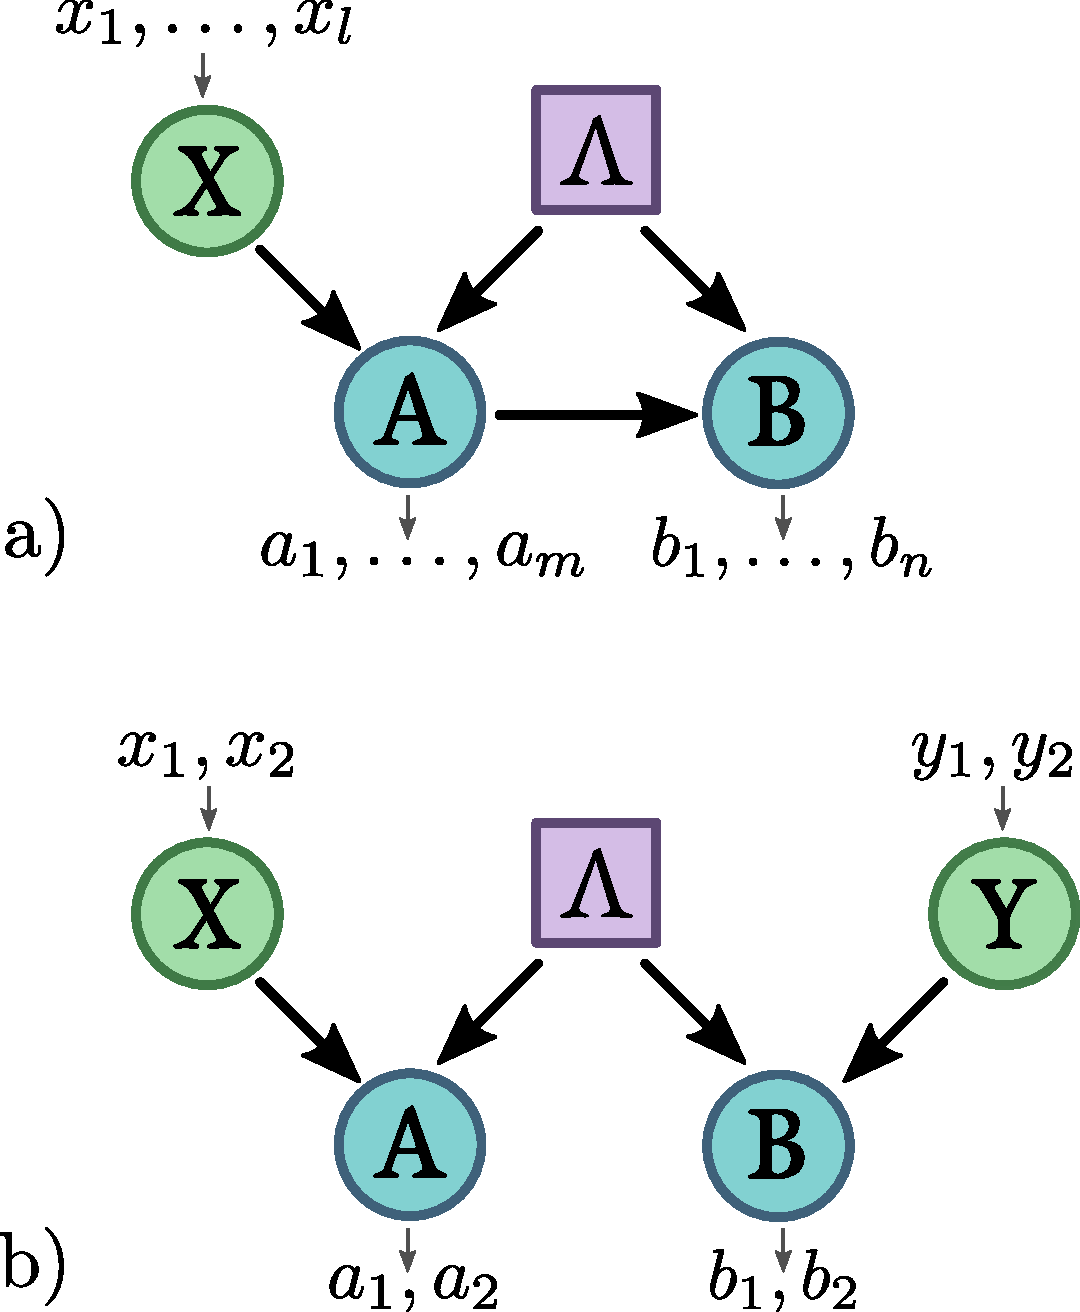
\includegraphics[width=.8\columnwidth]{images/chsh_inst_dag.pdf}
        \caption{
    \textbf{a)} The directed acyclic graph (DAG) representing a general
    Instrumental scenario, with $l$ possible values for the random variable $X$
    and $m,n$ possible outcomes for $A$ and $B$ respectively
    \textbf{b)} The directed acyclic graph (DAG) of the CHSH scenario where all the
    variables $X,Y,A$ and $B$ can only take two possible values.
}
    \label{fig:chshinstdag}

\end{figure} 

\section*{Instrumental variables, estimation of causal influences and a new form of quantum non-locality}

It has become standard to represent causal relations via directed acyclic graphs
(DAG), where the nodes represent random variables interconnected by directed
edges (arrows) accounting for their cause and effect relations \cite{pearlbook}.
A set of variables  $\left( X_1,\dots, X_n \right)$ form a Bayesian network with
respect to the graph if every variable $X_i$ can be expressed as a function of
its parents $PA_i$ and potentially an unobserved noise term $U_i$, such that
$U_i$ are jointly independent. This implies that the probability distribution of
such variables should have a Markov decomposition 
\footnote{Uppercase letters label variables and lowercase label the values taken
by them, for instance, $p(X_i =x_i, X_j = x_j) \equiv p(x_i, x_j)$.}
\begin{equation}
p(x_1,\dots,x_n)= \prod_{i=1}^{n} p(x_i \vert pa_i).    
\end{equation}
Importantly, a DAG typically implies non-trivial constraints over the
probability distributions that are compatible with it. That is, simply from
observational data and without the need of interventions, one can test whether
some observed correlations are incompatible with some causal hypothesis.

%and the edges the cause-effect relationship between them.
%From some causal DAGs it is possible to derive constraints on the statistical
%distribution of the variables which allow one to reject or accept a causal
%assumption\cite{pearlbook}.

Within this context, an important DAG is that corresponding to the instrumental
scenario (see Fig.\ref{fig:chshinstdag}-a). Following the Markov decomposition, any
empirical data encoded in the probability distribution $p(a,b \vert x)$ and
compatible with the instrumental causal structure can be decomposed as
\begin{equation}
p(a,b \vert x) = \sum_{\lambda} p(a\vert x,\lambda) p(b\vert a,\lambda)p(\lambda).
\end{equation}
Two causal assumptions are employed to arrive at the decomposition above. First,
the assumption that $p(x,\lambda)=p(x)p(\lambda)$, which implies the independence of
the instrument and the common ancestor. Second, the assumption that even though
$X$ and $B$ can be correlated, all these correlations are mediated by $A$. In
other terms, there is no direct causal influence between $X$ and $B$ and
$p(b\vert x,a,\lambda)=p(b\vert a,\lambda)$.

The instrumental variables have been originally introduced to estimate parameters
in econometric models of supply and demand \cite{economic} and, since then, have found a
wide range of applications in various other fields \cite{economic2, economic3}. To illustrate its
power, consider that variables $A$ and $B$ are related by a simple structural
equation $B=\gamma A +\Lambda$, where $\Lambda$ may represent a latent common
factor. By assumption, the instrumental variable $X$ should be independent of
$\Lambda$, thus implying that the causal strength can be estimated as $\gamma=
\mathrm{Cov}(X,B)/\mathrm{Cov}(X,A)$ where $\mathrm{Cov}(X,A)= \mean{X,A} -
\mean{X}\mean{A}$ is the covariance between $X$ and $A$. Strikingly, one can
estimate the causal strength even without any information about the latent
factor $\Lambda$. More generally and without assumptions about the functional
dependence among the variables, the empirical data encoded in the probability
distribution $p(a,b \vert x)$ can also be used to bound different quantifiers of
causality between $A$ and $B$ \cite{}.

%Among all the possible causal structures, a
%particular interest has been devoted to the %\textit{Instrumental causal
%structure} (see Fig.\ref{fig:chshinstdag}-a) introduced by Pearl\cite{pearl1995}
%in the 90's with applications ranging from econometrics[] to clinical trial[]. 
%One of the most important properties of instrumental variables is the fact that
%allow us to bound causal relations between variables solely from observational
%data. 
%Like in the Bell tests where the inequalities allow us to test local-realism for
%a particular distribution, instrumental inequalities test whether we have a
%valid instrument.
%Recently has been experimentally proved that instrumental inequalities are also
%violated when considering quantum resources \cite{chaves2018}, thus opening
%several venues for future research such as device-independent cryptography [],
%random number generation[] and basically any application that until now has been
%linked with the Bell scenario.
%In light of the importance regarding the instrumental causal structure, we are
%interested in exploring new techniques in order to better address the question
%of whether we can obtain a quantum violation, and what is the optimal test
%constrained on given experimental data.  

%Let us consider the intrumental structure depicted in Fig.\ref{fig:instdag}
%where X corresponds to the instrument, A and B the variables for which we are
%interested to bound the causal relation and $\Lambda$ our %quantum resource. 

Clearly, however, to draw any causal conclusions, first it is necessary to
certify that one has a valid instrument. This is achieved via instrumental
inequalities, first introduced by Pearl \cite{Pearl1995}. If we allow the variables $X$,
$A$, $B$ to take the values in the range  $x=1,\dots,l$, $a=1,\dots,m$ and
$b=1,\dots,n$ Pearl showed that the instrumental causal structure implies that 
\begin{equation} 
    \sum_{j=0}^{n} P(a_i b_j|x_{k(i,j)}) \le 1,
    \label{eq:pearl_ineq}
\end{equation}
for all $i \in {1,\ldots, m}$ and for all the possible functions $k(i,j)$ where $p(a=i,b=j\vert x=k)=p(a_i,b_j|x_k)$.

Extending these results, Bonet \cite{bonet2001} provided a 
general geometric framework for the derivation of instrumental inequalities.
Instrumental correlations define a convex set, a polytope described by finitely
many extremal points, or alternatively by a finite number of facets, among which, the
non-trivial are precisely the instrumental inequalities. In particular,
considering the case $(l,m,n) = (3,2,2)$, it was proven that there are two
inequivalent classes of instrumental inequalities (those not obtained from each
other by permuting the labels of $a_i,b_j$ and $x_k$). One class corresponding
to Pearl's inequality \eqref{eq:pearl_ineq} and the other given by
\begin{multline}
    P(a_1 b_1 | x_1) + P(a_2 b_2 | x_1) + 
    P(a_1 b_1 | x_2) +\\+ P(a_2 b_1 | x_2) + 
    P(a_1 b_2 | x_3) \le 2.
    \label{eq:bonet_ineq}
\end{multline}

All these conclusions and results, however, rely on a classical description of
causal and effect relations, that since Bell's theorem \cite{} we know do not
apply to the world governed by quantum mechanics. This has motivated the
question of whether many of the cornerstones in causal inference have to
reevaluated or reinterpreted in the presence of quantum effects \cite{}. Indeed,
as recently shown \cite{chaves2018}, violations of the instrumental tests are
possible even though the causal constraints underlying the instrumental scenario
are fulfilled. As shown in the experimental implementation of the instrumental
test \cite{chaves2018}, this is possible due to the presence of quantum entanglement
acting as latent common ancestor. Considering an entangled sources of photons,
an alternative version of Bonet's inequality (written in terms of expectation
values, upper bounded by 3, in the classical realm) has been tested, implying a
violation of the inequality \eqref{eq:bonet_ineq} with a 
value of $3.258 \pm 0.020$. 

Altogether, this shows the necessity of a new unifying framework, not only
considering what are the classical instrumental correlations but as well the
ones achievable if the underlying latent factor might have a quantum origin. In
the following we will achieve that by proposing a graph-theoretical approach to analyze the instrumental inequalities.

%\begin{equation}
%    -\avg{B}_{x_1} + 2 \avg{B}_{x_2} + %\avg{A}_{x_1} - \avg{AB}_{x_1} +
 %  2\avg{AB}_{x_3} \le 3  
  %  \label{eq:rafael_ineq}
%\end{equation}
%achieving a violation of $3.790 \pm 0.013$, translating to a violation of the original inequality \eqref{eq:bonet_ineq} with a 
%value of $2.159 \pm 0.005$. 

\section*{The exclusivity graph approach}

The graph-theoretical approach we propose here, was initially developed to the study of non-contextual inequalities \cite{cabello2014} as well as Bell non-locality scenarios \cite{acin2015} and obtain their quantum violation. In this formalism, every possible event, i.e. every possible set of measurement outcomes $a_1^,\ldots, a_n$ corresponding to given measurement settings $x_1,\ldots,x_n$ (each of which can be understood as an instrument), is associated to a vertex in a (undirected) graph $G = (V, E)$. Two vertices $u, v \in V$ are then connected by an edge $uv \in E$ if and only if they are exclusive, i.e.  if exists a measurement/instrument that can distinguish between them. Any linear constraint (like the instrumental inequalities) can be expressed defining a linear function 
\begin{equation}
    I_w(p) = \sum_{\substack{a_1,\ldots,a_n\\x_1,\ldots,x_n}}
w_{\substack{a_1,\ldots,a_n\\x_1,\ldots,x_n}} p(a_1,\ldots,a_n|x_1,\ldots,x_n)
\end{equation}
on the probabilities of possible events. This linear function can be represented by the weighted exclusivity graph $G$. Nicely, as it will be discussed below, bounds for the maximum values for $ I_w(p)$ achievable in classical and quantum physical theories can be related to two well-known graph invariants \cite{}: the independence number $\alpha(G, w)$ and the Lovász theta $\theta(G, w)$, respectively. In the following, we will briefly introduce these concepts and their interconnections, a more extensive and detailed account can be found in \cite{cabello2014, rabelo2014,acin2015}

Consider a graph $G(V,E)$ with vertex weights $w$, and $|V| = n$ .
We call a \emph{characteristic labelling} for $U \subseteq V$ a vector $x_v \in
\{0,1\}^n$ such that $x_v = 1$ if $v \in U$ and $x_v = 0$ otherwise.

An \emph{independent set} or \emph{stable set} is a set
$S \subset V$ such that $uv \notin E$ for all $u,v \in S$.
The independence number $\alpha(G, w)$ is defined as the maximum number of vertices (weighted with $w$) of an independent set of $G$. Is also customary to define the set $\STAB(G)$ as the convex hull of all the
characteristic labellings of stable sets:
\begin{equation} 
    \STAB(G) = \{x : x \quad \text{is a stable labelling of}\quad G \}.
    \label{eq:stab}
\end{equation}
Using this definition the independence number becomes:
\begin{equation}
    \alpha(G,w) = \max\{w\cdot x: x \in \STAB(G)\}
    \label{eq:alphastab}
\end{equation}
From these definitions, we can see that $\alpha(G,w)$ corresponds to the classical bound of the inequality, since it is exactly the maximum over the convex set defined by all the deterministic strategies respecting the exclusivity constraints.

We now call an \emph{orthonormal labelling} of dimension $d$ a map
$a_v:V \rightarrow \Real^d$ such that $a_v \cdot a_u = 0$ for all $uv \in E$ and
$|a_v|^2 = 1$, and we define the set $\TH(G)$ as:
\begin{multline}
    \TH(G) = \{x: x_v = (a_v)_1 \, \text{where $a_v$ is an} \\ \text{orthonormal labelling of $G$}\}
    \label{eq:thbody}
\end{multline}
It can be proved that this set includes all correlations permitted by quantum
theory\footnote{As proved in \cite{acin2015} this set corresponds to the level
$1+AB$ of the NPA (Navascués-Pironio-Acín) hierarchy \cite{npa2008}.}, % cite also almost-quantum correlations. 
but in general is larger as it contains correlations beyond those achieved by quantum
mechanics \cite{almostquantum2015}.
Maximizing over $\TH(G)$ gives the Lovász theta:
\begin{equation}
    \theta(G,w) = \{w\cdot x : x \in \TH(G)\}
    \label{eq:lovasztheta}
\end{equation}
which upper-bounds the maximum quantum value.
% EXPAND? when the almost quantum is = quantum
This approach provides a useful condition to check if a given graph $G$ admits a
quantum violation. Indeed it can be proven that $\TH(G) = \STAB(G)$ if and only
if $G$ does not contain a cycle $C_n$ with $n \ge 5$ and odd, or its complement
as an induced subgraph. This follows directly from the so called ``sandwich
theorem'' and the ``strong perfect graph theorem'' \cite{knuth}.
% EXPAND: some words on these 2 theorems

\section{Exclusivity graph method applied to causal models}
Next we show how the techniques presented in the previous section can be employed to analyze
a broad class of causal models. Consider a DAG as in fig~\ref{fig:onelambda}, with
$k$ observable variables $A_k$ with potential causal arrows among them, $l$
instruments $X_l$ with no incoming edges, and a single unobservable latent
variable $\Lambda$ acting as a potential common factor for all $A_k$ (but not to
$X_l$).

\begin{figure}[h]
    \centering
    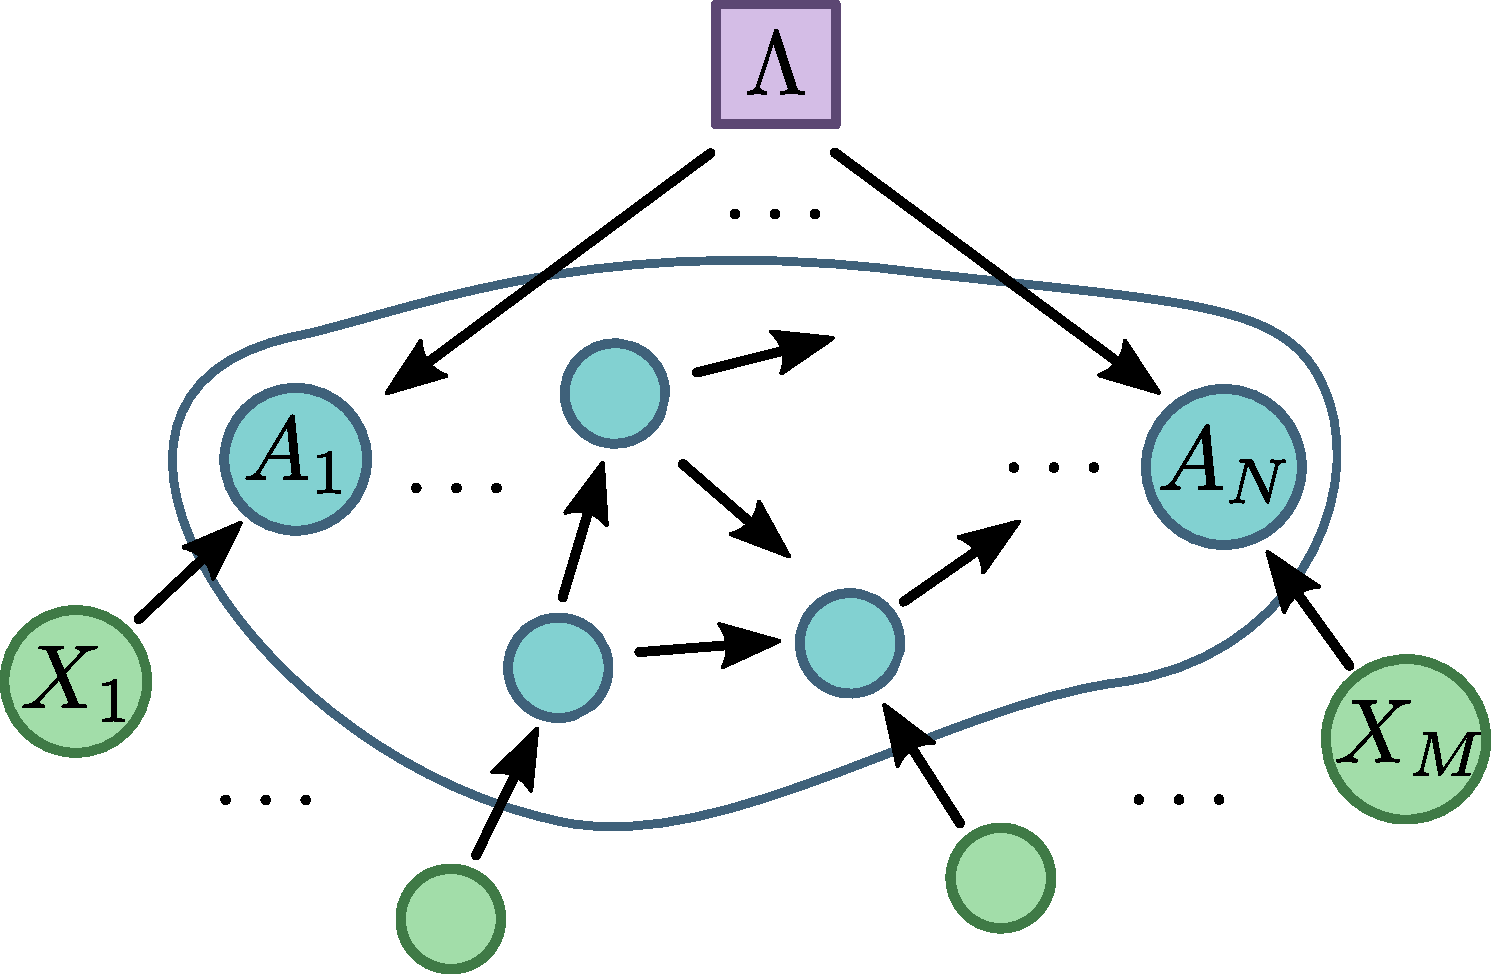
\includegraphics[width=.9\columnwidth]{images/onelambda.pdf}
    \caption{A represetantion of the class of causal structures to which our
    method can be applied.
    Those arewith $k$ observable variables, $l$ instruments and a single latent     variable.}
    \label{fig:onelambda}
\end{figure}

A \emph{non-exclusivity} graph can be associated with such a DAG
%(also called a \emph{confusability} graph) 
as follows:
\begin{itemize}
    \item Nodes are associated to events like $a | x$, where $a = (a_1,\ldots,a_k)$ and  $x = (x_1,\ldots,x_l)$.
    \item Two nodes $a | x $, and $a' | x'$ are linked by an edge if and only if 
        \begin{enumerate}
            \item for all $i,j \in \{1,\ldots,k\}$ if $A_i\,
                \rightarrow\, A_j$ then $\exists g_{ij} : g_{ij}(a_i) = a_j
                \et g_{ij}(a'_i) = a'_j$.
            \item for all $i\in \{1,\ldots,l\}$ and $j\in \{1,\ldots,k\}$ if
                $X_i\,\rightarrow\,A_j$ then $\exists f_{ij} : f_{ij}(x_i) = a_j
                \et f_{ij}(x'_i) = a'_j$.
        \end{enumerate}
\end{itemize}

As we will show next, considering the particular case of the instrumental
scenario \cite{}, one can apply the graph-theoretical methods delineated before
to the complement of this graph, $G=\bar{G}$, and its subgraphs. This allows to
obtain instrumental inequalities and their respective quantum and
classical bounds.

\subsection{The Instrumental exclusivity graph}
\begin{figure*}[t]
    \centering
    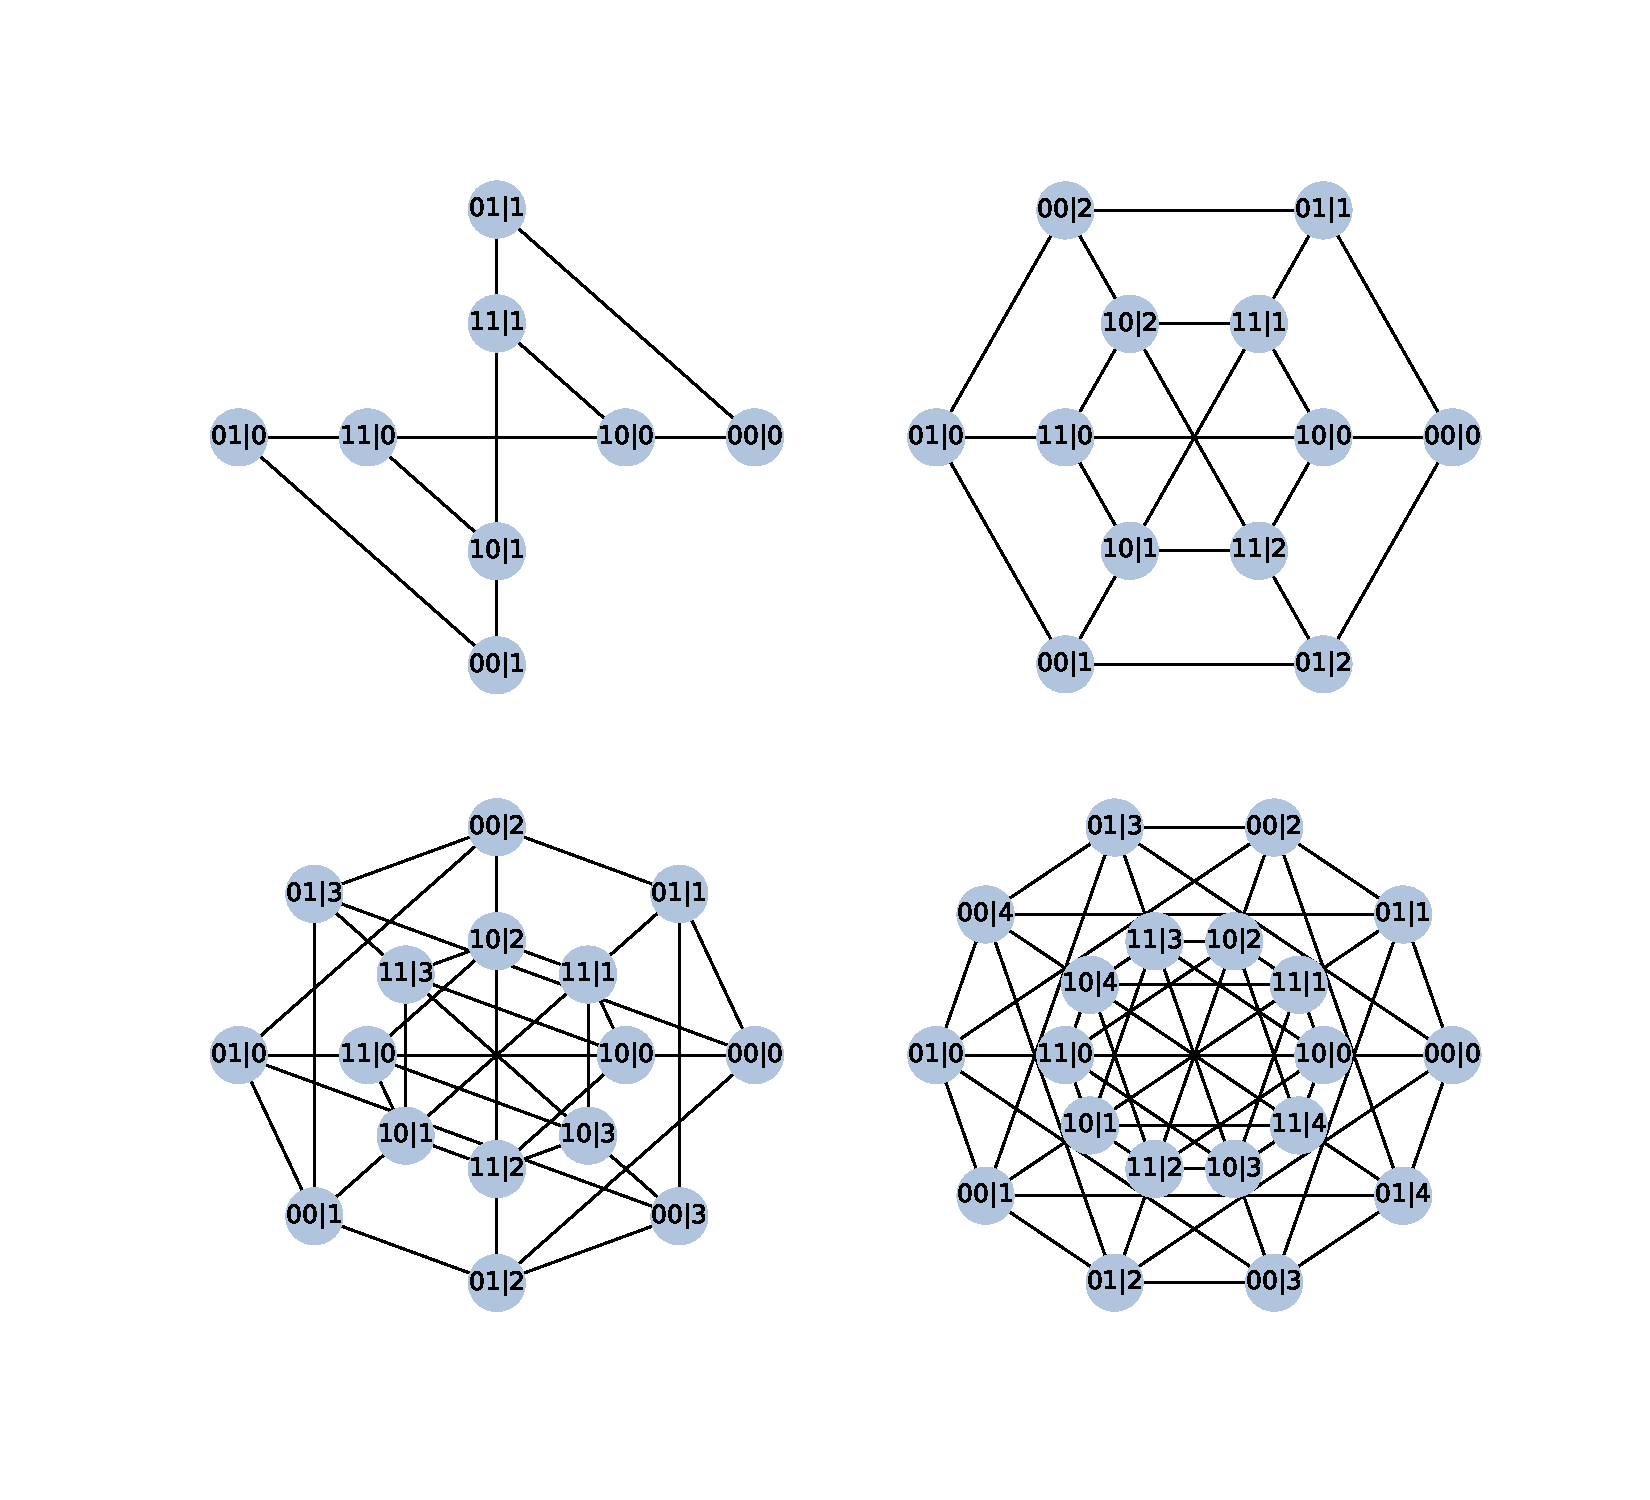
\includegraphics[width=.7\textwidth]{images/instrumental_exgraph.pdf}
    \caption{
    The exclusivity graph for the instrumental scenario $l22$ with $l=2,3,4,5$
    respectively from top left to bottom right. 
    To simplify the representation cliques are represented with the bold lines
    in the figure.}
    \label{fig:instrumental_exgraphs}
\end{figure*}

%Many known results about the instrumental scenario, including the inequality
%\eqref{eq:bonet_ineq}, can also be obtained using this formalism.

Without loss of generality we will restrict our attention to the case of
dichotomic observables ($n = m = 2$), considering $p(ab|x)$ with $a, b \in
\mathcal{A} = \mathcal{B} = \{0,1\}$ and $x \in
\mathcal{X} = \{0,\ldots,l\}$, the probability of having outcomes $a$ and $b$
with the instrument assuming the value $x$. As detailed above, the
non-exclusivity graph for the instrumental scenario is obtained by linking two
events $ab|x$ and $a'b'|x'$ if there exist two functions $f:\mathcal{X}
\rightarrow \mathcal{A}$ and $g:\mathcal{A} \rightarrow
\mathcal{B}$ such that:
\begin{eqnarray}
   & &  a = f(x) \quad\text{and}\quad a'=f(x')\\ \nonumber
& & b = g(a) \quad\text{and}\quad b'=g(a')
    \label{eq:non_exclusivity_condition}
\end{eqnarray}
As shown in figure \ref{fig:instrumental_exgraphs}, we construct the exclusivity
graphs for various $l$ and use the graph-theory methods described earlier to
obtain the classical and quantum bounds for several inequalities in the
instrumental scenario. 

First, consider the case $l=2$, for which Pearl's inequality (???) defines the
only instrumental inequality. It has been shown that this inequality does not
have a quantum violation \cite{}. For that, general probabilistic Bayesian
networks, including classical and quantum causal models as particular cases, had
to be introduced. In contrast, in our method it is straightforward not only to
derive the classical bound to Pearl's inequality 
%TODO: [Give more details about that 
but also to show that there is no quantum violation of the
inequality. This follows immediately from the fact that the corresponding
exclusivity graph (and its complement) does not contain any odd cyclic graph
with more than $5$ vertices, a necessary condition for any quantum violation.  

\begin{figure}[h]
    \centering
    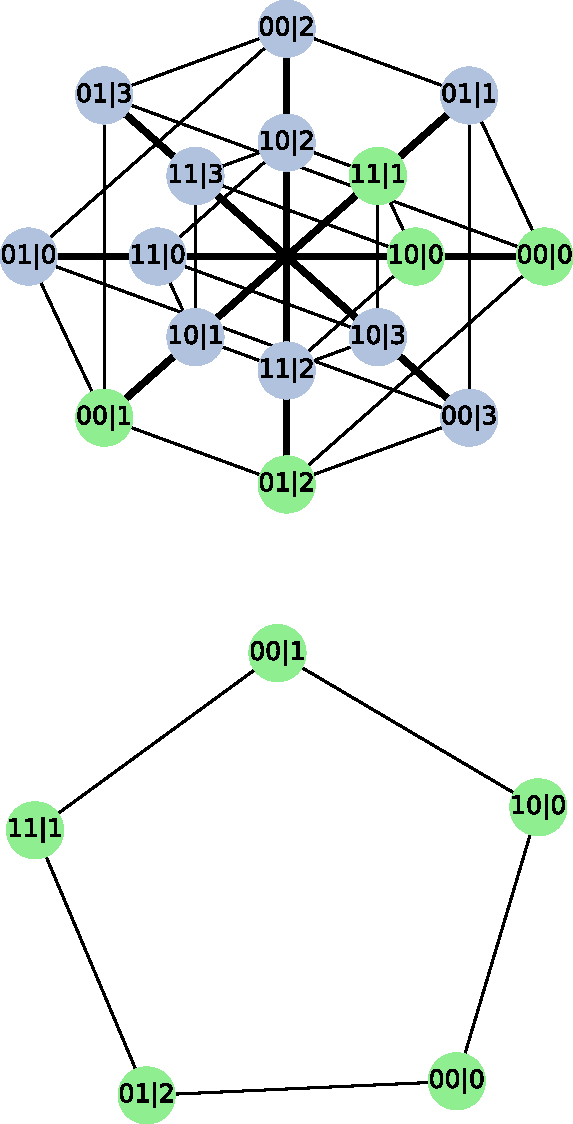
\includegraphics[width=.8\columnwidth]{images/instrumental_c5.pdf}
    \caption{The exclusivity graph of the bonet inequality, as an induced
    subgraph of complete one of the $322$ instrumental scenario.}
    \label{fig:bonetexc}
\end{figure}

For $l\ge3$ we see that there might be a quantum violation, since the associated graph has as a subset a $C_5$ cyclic graph, i.e. the pentagon depicted in
fig.~\ref{fig:bonetexc} that is exactly the Bonet's inequality \eqref{eq:bonet_ineq}.
For cyclic graphs it is known that $\alpha(C_n) = \lfloor n/2 \rfloor$ and
$\theta(C_n) = n\cos(\pi/n)/(1+\cos(\pi/n))$. For $n=5$, it follows directly the
gap between the classical and quantum theories, since the classical limit is
given by $\alpha(C_5)=2$ and the quantum one given by $\theta(C_5)=\sqrt{5}$.
%\textcolor{red}{I'm a bit confused... the maximum quantum violation of the
%Bonet's inequality is $\sqrt{5}$ or $(3+\sqrt{2})/2$? Explain this a bit
%better...}
% EXPAND: how to get the quantum bound.

In this framework, Eq. \eqref{eq:bonet_ineq} seems analogous to the KCBS contextual
inequality\cite{kcbs2008}.
The difference here is that the quantum limit is not $\sqrt{5}$, which we cannot
obtain in a bipartite scenario.
To find a tight bound we must apply other methods to our graph, like the ones in
\cite{rabelo2014}, which bring $(3+\sqrt{2})/2$.

As it will be shown below, no other odd anticycle besides
$C_5$ is present for any $l$, that is, if we increase the cardinality of the
instrumental variable. 
%From this point of view, we can say that any quantum violation for a general
%$l22$ instrumental scenario has essentially the same origin: it stems from the
%non classicality of the $C_5$ graph. 
%\textcolor{red}{[]Can we say that? What about the other kind of inequality discussed below?]}

This does not mean that different inequalities cannot be devised by clever
choices of vertices and weights. 
%\textcolor{red}{[]Is there any algorithm for
%that? Or is really trial and error? I'm confused by the method... are you
%combining the two graphs to construct a single inequality?]}
For example, in the $422$ scenario  we can find the following inequality:
%\begin{equation}
 %   \avg{AB}_1 -  \avg{AB}_2 + \avg{B}_0 - \avg{B}_3 \le 2
  %  \label{eq:422_ineq}
%\end{equation}
\begin{multline}
    p(00|10) + p(11|11) + p(01|20) + p(10|21) +\\
    + p(00|00) + p(10|01) + p(01|30) + p(11|31) +\\
    - p(01|10) - p(10|11) - p(00|20) - p(11|21) +\\
    - p(01|00) - p(11|01) - p(00|30) - p(10|31)
    \le 2
    \label{eq:422_ineq}
\end{multline}

Eq. \ref{eq:422_ineq} corresponds to the two sets of events whose
exclusivity graphs are depicted in fig.~\ref{fig:422_exgraph}.
The maximum classical value for both graph, given by their independence numbers, is $3$, while their minimum is $1$, which gives the maximum value of $2$
as in \eqref{eq:422_ineq} when taken with opposite sign.
This inequality has a structure very similar to the CHSH (showed in
fig.\ref{fig:chsh_exgraph}), and, as pointed out above, both arise from the
non-classicality of the $C_5$ graph.

\begin{figure}[b]
    \centering
    \parbox{.9\columnwidth}{
        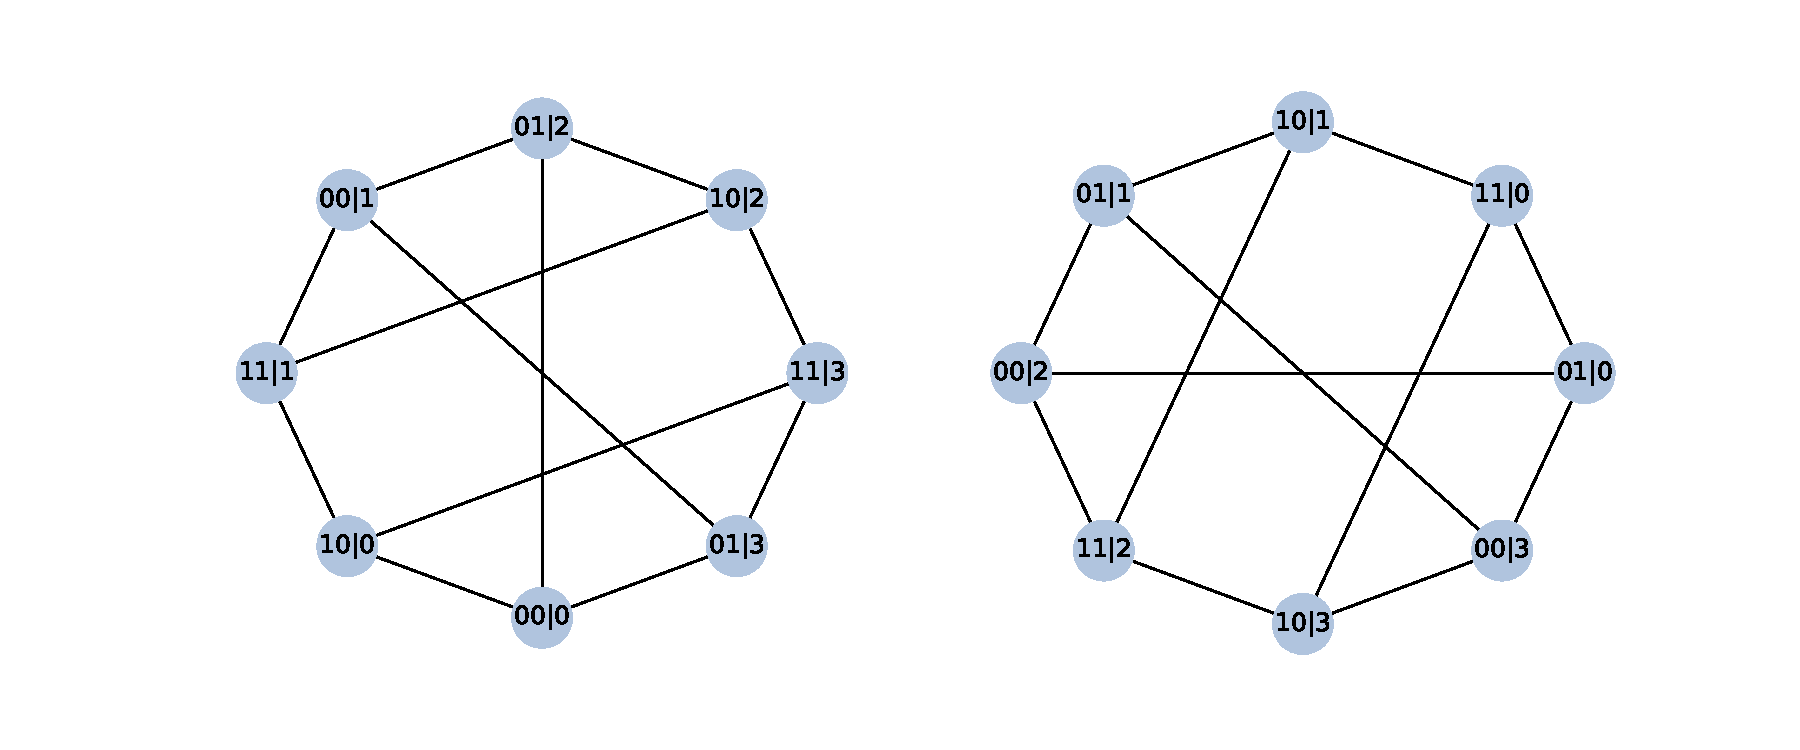
\includegraphics[width=\columnwidth]{images/422_exgraph.pdf}
        \caption{The exclusivity graph for the $422$ Instrumental scenario.}
        \label{fig:422_exgraph}
    }

    \bigskip
    \parbox{.9\columnwidth}{
        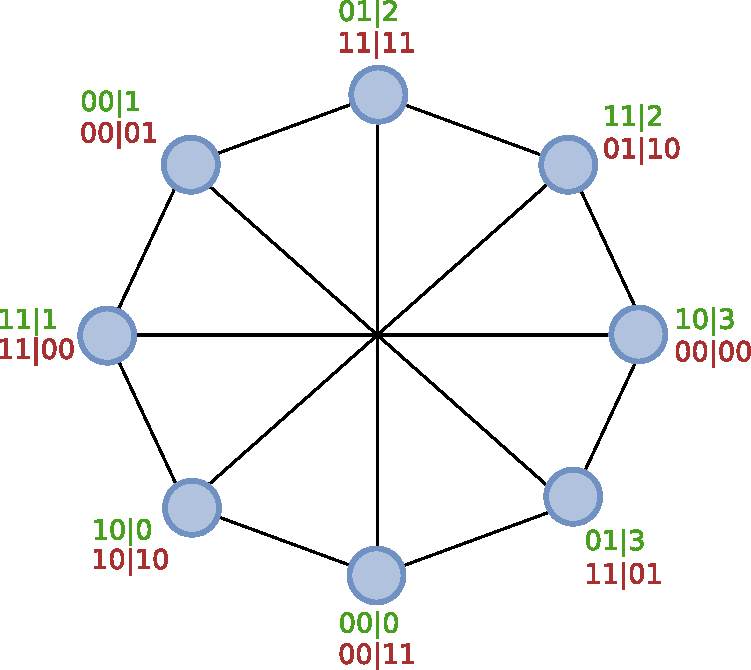
\includegraphics[width=\columnwidth]{images/gclmp_graphs.pdf}
        \caption{The exclusivity graphs for the the CHSH inequality in the Bell
        scenario.}
        \label{fig:chsh_exgraph}
    }
\end{figure}



%\section{Finding optimal instrumental inequalities}
%The presence of an odd cycle graph guarantees only that $\STAB(G) \subset
%\TH(G)$, but does not say anything on the %values of $\theta(G)$ and $\alpha(G)$.
%Nonetheless, if that condition is %satisfied there must be some optimal %choice of
%weights $w$ for which we can obtain a %maximum quantum violation.
%Formally if $n$ is the number of nodes of %$G$, we want to find the maximum:
%\begin{equation}
%    \max_{w \in [0,1]^n} \{\theta(G,w) - %\alpha(G,w)\}
%    \label{eq:maxonw}
%\end{equation}
%
%Using the definition \eqref{eq:lovasztheta} and \eqref{eq:alphastab}, and
%remembering that $\STAB(G)$ is a convex %hull of a finite number of
%characteristic labellings we can rewirte %the previous maximization as:
%\begin{align}
%    \Delta &= \min \{I_y : y \, \text{is a %maximal stable labelling}\}
%    \label{eq:maximize_w_delta}\\
%    I_y &= \max_{\substack{w \in %[0,1]^n\\x \in \TH(G)}} \{w\cdot (x - %y)\}
%    \label{eq:maximize_w_I}
%\end{align}
%
%The maximization \eqref{eq:maximize_w_I} %for each $y$ is efficient, being a
%semi-definite program, but unfortunately %it has to be run for each maximal
%stable set in $G$ which are $\sim 3^{n/3}$ %in the worst case.
%Also to enumerate all the maximal %independent sets we used the Tomita %version of
%the Bron–Kerbosch algorithm which has the %same worst case
%complexity\cite{tomita2006}.
%
\section*{Discussion}

%TODO: add an example with more outcomes

\subsubsection*{Acknowledgements}
We acknowledge support from John Templeton Foundation via the grant Q-CAUSAL
n$^{\circ}$61084 (the opinions expressed in this publication are those of the
    authors and do not necessarily  the views of the John Templeton
Foundation). RC acknowledges the Brazilian ministries MEC and MCTIC, funding
agency CNPq (PQ grants No. 307172/2017-1 and No 406574/2018-9 and INCT-IQ) and
the Serrapilheira Institute (grant number Serra-1708-15763).

\section*{Methods}
\subsection*{There are no cycles $C_n$ with $n \ge 7$ in the $d22$ instrumental scenario.}
%\label{sec:c5only_proof}
In the following we prove that there cannot be a odd anticycle with more than
$5$ vertices in the exclusivity graph associated to an instrumental scenario of
the type $d22$.

\begin{figure}[h]
    \centering
    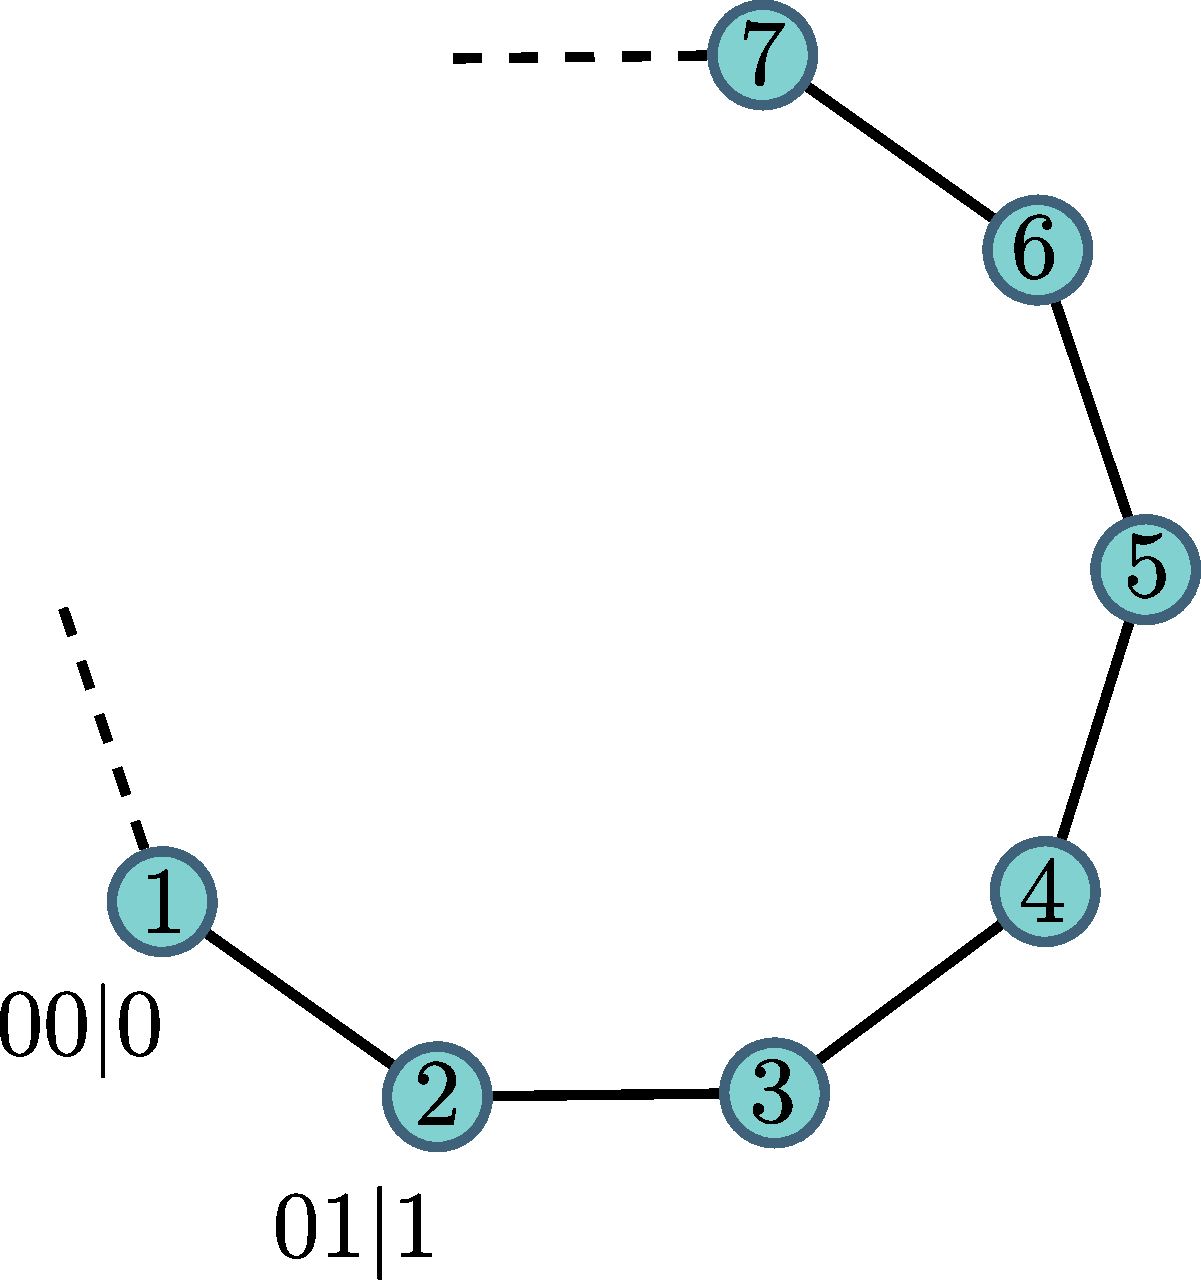
\includegraphics[width=.6\columnwidth]{images/cycle_proof.pdf}
    \caption{Proof of the impossibility of having cycles with $7$ nodes or more
    in the $d22$ scenario.}
    \label{fig:cycle_graph_proof}
\end{figure}

From the exclusivity conditions \eqref{eq:non_exclusivity_condition},
given two events $ab|x$ and $a'b'|x'$, they are connected by edge if one of these two conditions is true:
\begin{enumerate}
    \item $x=x'$.\label{en:rule1}
    \item $a=a'$ and $b \neq b'$.\label{en:rule2}
\end{enumerate}
Suppose we have a cycle $C_n$ with $n \ge 7$, as in fig.~\ref{fig:cycle_graph_proof},
and consider that node $2$ in this graph corresponds to an event which we can arbitrarily identify as $00|0$.
Among its neighbors $1$ and $3$, one will necessarily need to satisfy rule
\ref{en:rule2} (they cannot both satisfy rule \ref{en:rule1} or the three nodes
would be a clique 
%TODO: Explain what is a clique.
So without loss of generality we can assign the event $01|1$ to $3$.
Since nodes $5,6,7$ must not satisfy rule \ref{en:rule2} with both $2$ and $3$, then they must have $a = 1$.
Moreover $7$ and $5$ must have the same $b$, different from $6$. In the same way $1$ must not satisfy rule \ref{en:rule2} with $6,5$ and $3$, so it
needs to have $a=0$ and $b=1$. At this point, since we only have values
$\{0,1\}$ for $a$, we cannot avoid node $4$ to be linked to one of the nodes
$1,2,6,7$. Thus, the corresponding graph cannot be a cycle.

\begin{thebibliography}{}
    \bibitem{pearlbook} J. Pearl, 
        {\em Causality: models, reasoning, and inference.}
        Cambridge University Press, (2000).
    \bibitem{pearl1995} J. Pearl, 
        {\em On the testability of causal models with latent and instrumental variables}, 
        Proceedings of the Eleventh conference on Uncertainty in artificial
        intelligence. Morgan Kaufmann Publishers Inc. (1995).
    \bibitem{bonet2001} B. Bonet, {\em Instrumentality tests revisited},
        Proceedings of the Seventeenth conference on Uncertainty in artificial
        intelligence. Morgan Kaufmann Publishers Inc. (2001).
    \bibitem{chaves2018} R. Chaves, G. Carvacho, I. Agresti, V. Di Giulio, L. Aolita,
        S. Giacomini, F. Sciarrino, 
        {\em Quantum violation of an instrumental test}, 
        Nature Physics 14.3 291 (2018).
     \bibitem{himbeeck2018} T. Van Himbeeck, J. B. Brask, S. Pironio, R. Ramanathan, A. B. Sainz, E. Wolfe, 
        {\em Quantum violations in the Instrumental scenario and their relations to the Bell scenario},
    \bibitem{economic} P. G. Wright, \emph{The tariff on animal and vegetable oils}, The Macmillan Company, (1928).
    \bibitem{economic2} C. W. J. Granger, \emph{Investigating causal relations by econometric models and cross-spectral methods}, Econometrica, 424 (1969).
    \bibitem{economic3} N. Cartwright, \emph{Causal Structures in Econometrics:On the Reliability of Economic Models},Recent Economic Thought Series \textbf{42}, pp 63-89 (1995).
        arXiv preprint arXiv:1804.04119 (2018).
     \bibitem{cabello2014} A. Cabello, S. Severini, A. Winter,
         {\em Graph-theoretic approach to quantum correlations}, 
         Physical review letters, 112(4), 040401 (2014).
     \bibitem{rabelo2014} R. Rabelo, C. Duarte, A. J.  López-Tarrida, M. T. Cunha, A. Cabello, A. 
         {\em Multigraph approach to quantum non-locality},
         Journal of Physics A: Mathematical and Theoretical, 47(42), 424021
         (2014).
     \bibitem{kcbs2008} A. A. Klyachko, M. A. Can, S. Binicioğlu, A. S. Shumovsky.
         {\em Simple test for hidden variables in spin-1 systems.}
         Physical review letters, 101(2), 020403 (2008).
     \bibitem{almostquatum2015} M. Navascués, Y. Guryanova, M. J. Hoban, \& A. Acín, 
         {\em Almost quantum correlations.}
         Nature Communications 6, (2015).
     \bibitem{npa2008} M. Navascués, S. Pironio, \& A Acín, 
         {\em A convergent hierarchy of semidefinite programs characterizing the
         set of quantum correlations.}
         New Journal of Physics 10, 073013 (2008).
     \bibitem{tomita2006} E. Tomita, A. Tanaka, \& H. Takahashi,
         {\em The worst-case time complexity for generating all maximal cliques
         and computational experiments.} 
         Theoretical Computer Science 363, 28–42 (2006).
         
         
         
         
         

%%%%%%%%%%%%%%%%%%%%%%%%%%%%%%%%%%%%%%%%%%%%%%%%%%%%%%%%%%%%%%%%%%%%%%%%%%%% (beta)


%\bibitem{clinical}K. Fischer and I. R. White, \emph{Causal Inference in Clinical Trials}, Wiley-Blackwell, (2012).

%\bibitem{genetic1}N. Friedman, \emph{Inferring cellular networks using probabilistic graphical models}, Science \textbf{303}, 799–805 (2004).

%\bibitem{genetic2}C. R. Shalizi and A. C. Thomas, \emph{Homophily and contagion are generically confounded in observational social network studies}, Sociological methods and research \textbf{40}, 211 (2011).

%\bibitem{social1}H. E. Brady, \emph{Causation and explanation in social science}, Oxford University press (2013).

%\bibitem{machle}D. Barber, \emph{Bayesian reasoning and machine learning}, Cambridge University press (2012).

%%%%%%%%%%%%%%%%%%%%%%%%%%%%%%%%%%%%%%%%%%%%%%%%%%%%%%%%%%%%%%%%%%%%%%%%%%%%%%%%%%

         
         
         
         
         
         
         
%\bibitem{} , {\em },  ().
\end{thebibliography}

%\begin{figure}[h]
%\vspace{1in}
%\caption{Sample Figure Caption}
%\end{figure}

\end{document}
